\documentclass[aspectratio=169, 10pt]{beamer}
\usetheme{Madrid}
\usefonttheme{professionalfonts}

\usepackage[utf8]{inputenc}
\usepackage[english]{babel}
\usepackage[linguistics]{forest}
\usepackage{algorithmic}
\usepackage{amsfonts}
\usepackage{amsmath}
\usepackage{amssymb}
\usepackage{array}
\usepackage{bookmark}
\usepackage{caption}
\usepackage{colortbl}
\usepackage{csquotes}
\usepackage{graphicx}
\usepackage{hyperref}
\usepackage{lipsum}
\usepackage{lmodern}
\usepackage{mathptmx}
\usepackage{mathtools}
\usepackage{svg}
\usepackage{xcolor}
\usepackage{multirow}

\hypersetup{
    colorlinks=true,
    linkcolor=blue,
    filecolor=blue,      
    urlcolor=blue,
}

\title{Tutorial 2}
\subtitle{Decision Tree, Cross-validation, Precision and Recall}
\author{Luke Chang}
\institute{The University of Auckland}
\date{Mar. 2021}


\begin{document}

\frame{\titlepage}

%-------------------------------------------------------------------------------
\begin{frame}
    \frametitle{Objectives}
    
    \begin{enumerate}
        \item Evaluation Metrics: Accuracy, Precision, Recall and F1 score
        \item ROC curve and AUC
        \item Should you trust the results?
        \item Parametric Tests VS. Non-parametric Tests
        \item Regression and Least Square Problem
        \item Ensemble Methods
    \end{enumerate}
    
\end{frame}

%-------------------------------------------------------------------------------
\begin{frame}
    \frametitle{Confusion Matrix}
    
    Confusion Matrix can be applied to \textbf{binary} classification as well as for \textbf{multiclass} classification problems.
            
    \begin{table}[]
        \begin{tabular}{cccc}
                                         &                                        & \multicolumn{2}{c}{\textbf{Predicted}}                                    \\
                                         &                                        & \textbf{Positive}                   & \textbf{Negative}                   \\ \cline{3-4} 
        \multirow{2}{*}{\textbf{Actual}} & \multicolumn{1}{c|}{\textbf{Positive}} & \multicolumn{1}{c|}{\cellcolor{blue!25}True Positive}  & \multicolumn{1}{c|}{\cellcolor{red!25}False Negative} \\ \cline{3-4} 
                                         & \multicolumn{1}{c|}{\textbf{Negative}} & \multicolumn{1}{c|}{\cellcolor{red!25}False Positive} & \multicolumn{1}{c|}{\cellcolor{blue!25}True Negative}  \\ \cline{3-4} 
        \end{tabular}
    \end{table}

    \begin{itemize}
        \item True Positive (TP): Correctly classified.
        \item True Negative (TN): Correctly rejected.
        \item False Positive (FP): Incorrectly classified. Type I Error.
        \item False Negative (FN): Incorrectly rejected. Type II Error.
    \end{itemize}

    \[
        \text{Accuracy} = \frac{\text{TP} + \text{TN}}{\text{TP} + \text{TN} + \text{FP} + \text{FN}}
    \]

\end{frame}

%-------------------------------------------------------------------------------
\begin{frame}
    \frametitle{Confusion Matrix}

    How many selected items are relevant? $\text{Selected Elements} = \text{TP}+ \text{FP}$
    \[
        \text{Precision (P)} = \frac{\text{TP}}{\text{TP}+ \text{FP}}
    \]

    How many relevant items are selected? $\text{Relevant Elements} = \text{TP}+ \text{FN}$
    \[
        \text{Recall (R)} = \frac{\text{TP}}{\text{TP}+ \text{FN}}
    \]
    
    $F_1$ score is the \textbf{harmonic mean} between Precision and Recall.

    \[
        F_1 = 2 \times \frac{P \times R}{P + R}
    \]
    
\end{frame}

%-------------------------------------------------------------------------------
\begin{frame}
    \frametitle{Example -- Weather Prediction}
    \begin{columns}
        \begin{column}{0.5\textwidth}
            Build a logistic regression model to predict the weather based on the humidity. \\
            Recorded 10 days in total.
            \begin{table}[]
                \begin{tabular}{cc}
                \textbf{Class} & \textbf{Prediction} \\ \hline
                P              & P                   \\
                N              & P                   \\
                P              & N                   \\
                P              & P                   \\
                N              & P                   \\
                P              & P                   \\
                N              & P                   \\
                N              & N                   \\
                N              & N                   \\
                P              & P                  
                \end{tabular}
            \end{table}

            \textbf{Caveat:} A model with high Recall may also has high FPR (Type I Error).

        \end{column}
        \begin{column}{0.5\textwidth}
            \begin{table}[]
                \begin{tabular}{ccccc}
                \textbf{}                        & \textbf{}                       & \multicolumn{2}{c}{\textbf{Predicted}}          &                \\
                                                 &                                 & \textbf{P}             & \textbf{N}             & \textbf{Total} \\ \cline{3-4}
                \multirow{2}{*}{\textbf{Actual}} & \multicolumn{1}{c|}{\textbf{P}} & \multicolumn{1}{c|}{4} & \multicolumn{1}{c|}{1} & 5              \\ \cline{3-4}
                                                 & \multicolumn{1}{c|}{\textbf{N}} & \multicolumn{1}{c|}{3} & \multicolumn{1}{c|}{2} & 5              \\ \cline{3-4}
                                                 & \textbf{Total}                  & 7                      & 3                      & \textbf{10}   
                \end{tabular}
            \end{table}
            
            \[
                \text{Acc.} = \frac{6}{10} = 0.6
            \]

            \[
                \text{Precision (P)} = \frac{\text{TP}}{\text{TP}+ \text{FP}} = \frac{4}{4+3} \approx 0.571
            \]

            \[
                \text{Recall (R)} = \frac{\text{TP}}{\text{TP}+ \text{FN}} = \frac{4}{4+1} \approx 0.8
            \]

            \[
                F_1 = 2 \frac{P \times R}{P + R} = 2 \times \frac{0.571 \times 0.8}{0.571 + 0.8} \approx 0.667
            \]

        \end{column}
    \end{columns}

\end{frame}

%-------------------------------------------------------------------------------
\begin{frame}
    \frametitle{Precision-Recall (PR) Curve (Optional)}
    
    Average precision (AP) summarizes such a plot as the weighted mean of precisions achieved at each threshold.
    \[
        AP = \sum_{n}(R_n - R_{n-1})P_n
    \]

    \begin{itemize}
        \item Where $P_n$ and $R_n$ are the precision and recall at the n-th threshold.
        \item A pair $(P_n, P_k)$ is referred to as an \textit{operating point}.
    \end{itemize}
    
    \begin{figure}
        \centering
        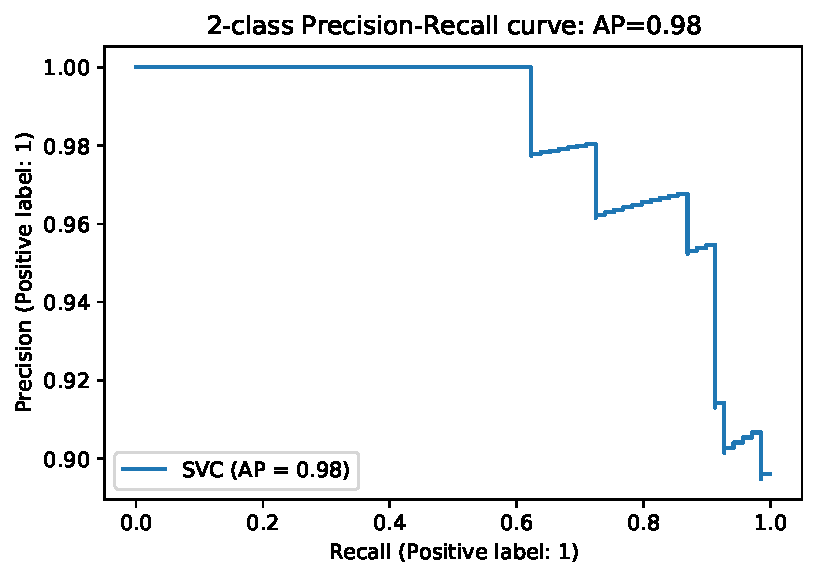
\includegraphics[width=0.35\columnwidth]{../plots/pr_curve.pdf}
        \caption{A SVM classifier trained on the Breast Cancer dataset}
    \end{figure}
\end{frame}

%-------------------------------------------------------------------------------
\begin{frame}
    \frametitle{Receiver Operating Characteristic (ROC) Curve}
    
    \begin{itemize}
        \item The ROC curve is created by plotting the true positive rate (TPR) against the false positive rate (FPR) at various threshold settings.
        \item Area Under Curve (AUC): The integration of the ROC function between 0 and 1.
    \end{itemize}
    
    \begin{figure}
        \centering
        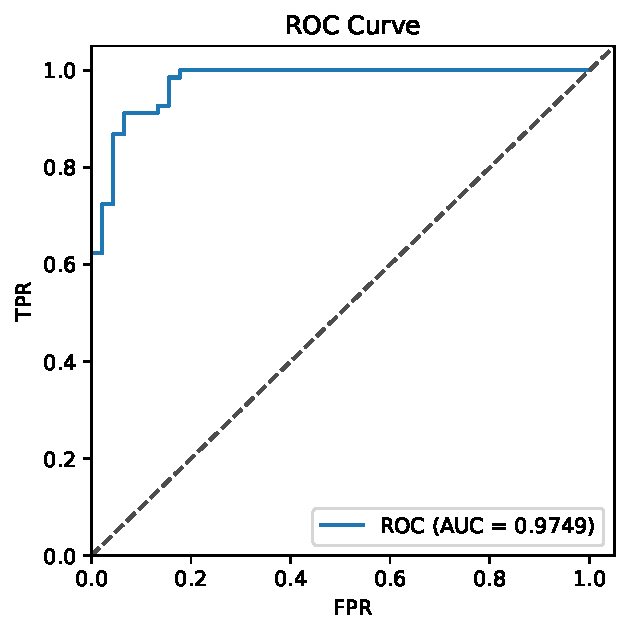
\includegraphics[width=0.3\columnwidth]{../plots/roc_curve.pdf}
        \caption{A SVM classifier trained on the Breast Cancer dataset}
    \end{figure}

\end{frame}

%-------------------------------------------------------------------------------
\begin{frame}
    \frametitle{Example -- Weather Prediction}
    
    \begin{columns}
        \begin{column}{0.5\textwidth}
            Build a logistic regression model to predict the weather based on the humidity. \\
            Recorded 10 days in total.
            
            \begin{table}[]
                \begin{tabular}{cc|cccccc}
                \textbf{}      & \textbf{}           & \multicolumn{6}{l}{\textbf{Thresholds}}                                             \\
                \textbf{Class} & \textbf{Prediction} & \textbf{0} & \textbf{0.2} & \textbf{0.4} & \textbf{0.6} & \textbf{0.8} & \textbf{1} \\ \hline
                P              & 0.95                & 1          & 1            & 1            & 1            & 1            & 0          \\
                N              & 0.85                & 1          & 1            & 1            & 1            & 1            & 0          \\
                P              & 0.78                & 1          & 1            & 1            & 1            & 0            & 0          \\
                P              & 0.66                & 1          & 1            & 1            & 1            & 0            & 0          \\
                N              & 0.6                 & 1          & 1            & 1            & 1            & 0            & 0          \\
                P              & 0.55                & 1          & 1            & 1            & 0            & 0            & 0          \\
                N              & 0.53                & 1          & 1            & 1            & 0            & 0            & 0          \\
                N              & 0.52                & 1          & 1            & 1            & 0            & 0            & 0          \\
                N              & 0.51                & 1          & 1            & 1            & 0            & 0            & 0          \\
                P              & 0.4                 & 1          & 1            & 1            & 0            & 0            & 0         
                \end{tabular}
                \end{table}

        \end{column}
        \begin{column}{0.5\textwidth}
            
            \begin{table}[]
                \begin{tabular}{c|cccccc}
                \textbf{Threshold} & \textbf{0} & \textbf{0.2} & \textbf{0.4} & \textbf{0.6} & \textbf{0.8} & \textbf{1} \\ \hline
                \textbf{TPR}       & 1          & 1            & 1            & 0.60         & 0.2          & 0          \\
                \textbf{FPR}       & 1          & 1            & 1            & 0.4          & 0.2          & 0         
                \end{tabular}
            \end{table}
            
        \end{column}
    \end{columns}
\end{frame}

%-------------------------------------------------------------------------------
\begin{frame}
    \frametitle{Should you trust the results?}
    
    
\end{frame}

%-------------------------------------------------------------------------------
\begin{frame}
    \frametitle{Parametric Tests VS. Non-parametric Tests}
    
    
\end{frame}

%-------------------------------------------------------------------------------
\begin{frame}
    \frametitle{Regression and Least Square Problem}
    
    
\end{frame}

%-------------------------------------------------------------------------------
\begin{frame}
    \frametitle{Ensemble Methods}
    
    
\end{frame}

\end{document}
